In this section I explore four methods of dimensionality reduction on both of my datasets.

\subsection{Principal Components Analysis}\label{subsec:principal-components-analysis}
\begin{center}
    \begin{tabular}{|c| c |c|}
        \hline
        & Minimum Components to Explain 99.9\% Variance & Eigenvalues                               \\
        \hline
        \hline
        Dataset 1 & 2                                             & [11320901200.524, 54484006.504]           \\
        \hline
        Dataset 2 & 4                                             & [65088.565, 37527.175, 4525.986, 106.278] \\
        \hline
    \end{tabular}
\end{center}
Two features explain 100\% of the variance in the data in the case of PCA for dimensionality reduction, and four features explain
99.9\% of the variance in the case of the second dataset.
In the case of dataset one the eigenvalues are very large which would seem to imply that the data are close together and
the are being multiplied by a large number to separate.
Figures~\ref{Fig:PCA DS1} and~\ref{Fig:PCA DS2} show the projection of the transformed data according to their principal
components for the first two features (to allow for plotting).
\begin{figure}
    \begin{minipage}{0.5\textwidth}
        \centering
        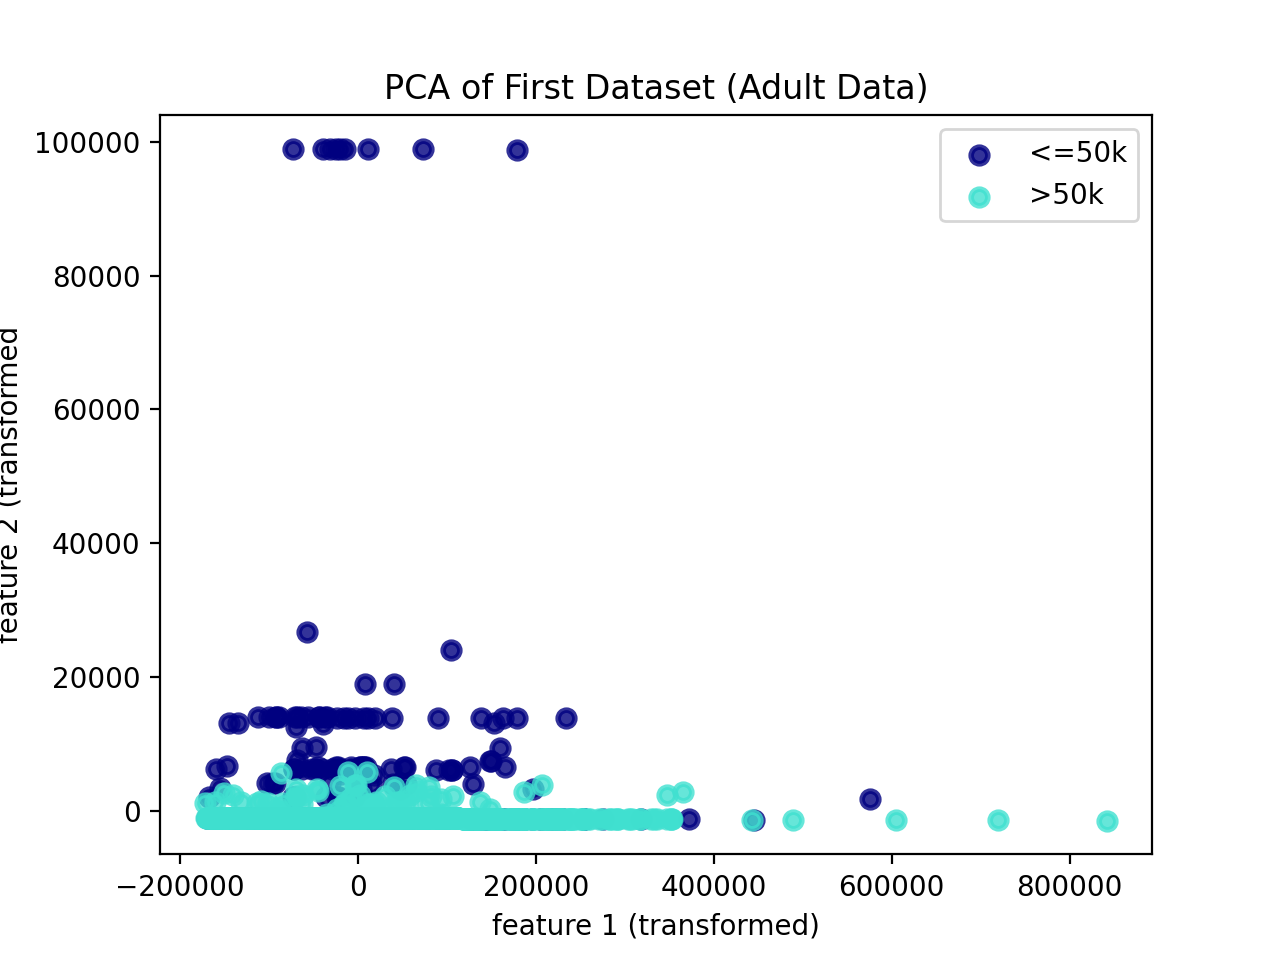
\includegraphics[width=.9\linewidth]{pcads1.png}
        \caption{DS1 Projection via PCA}\label{Fig:PCA DS1}
    \end{minipage}\hfill
    \begin{minipage}{0.5\textwidth}
        \centering
        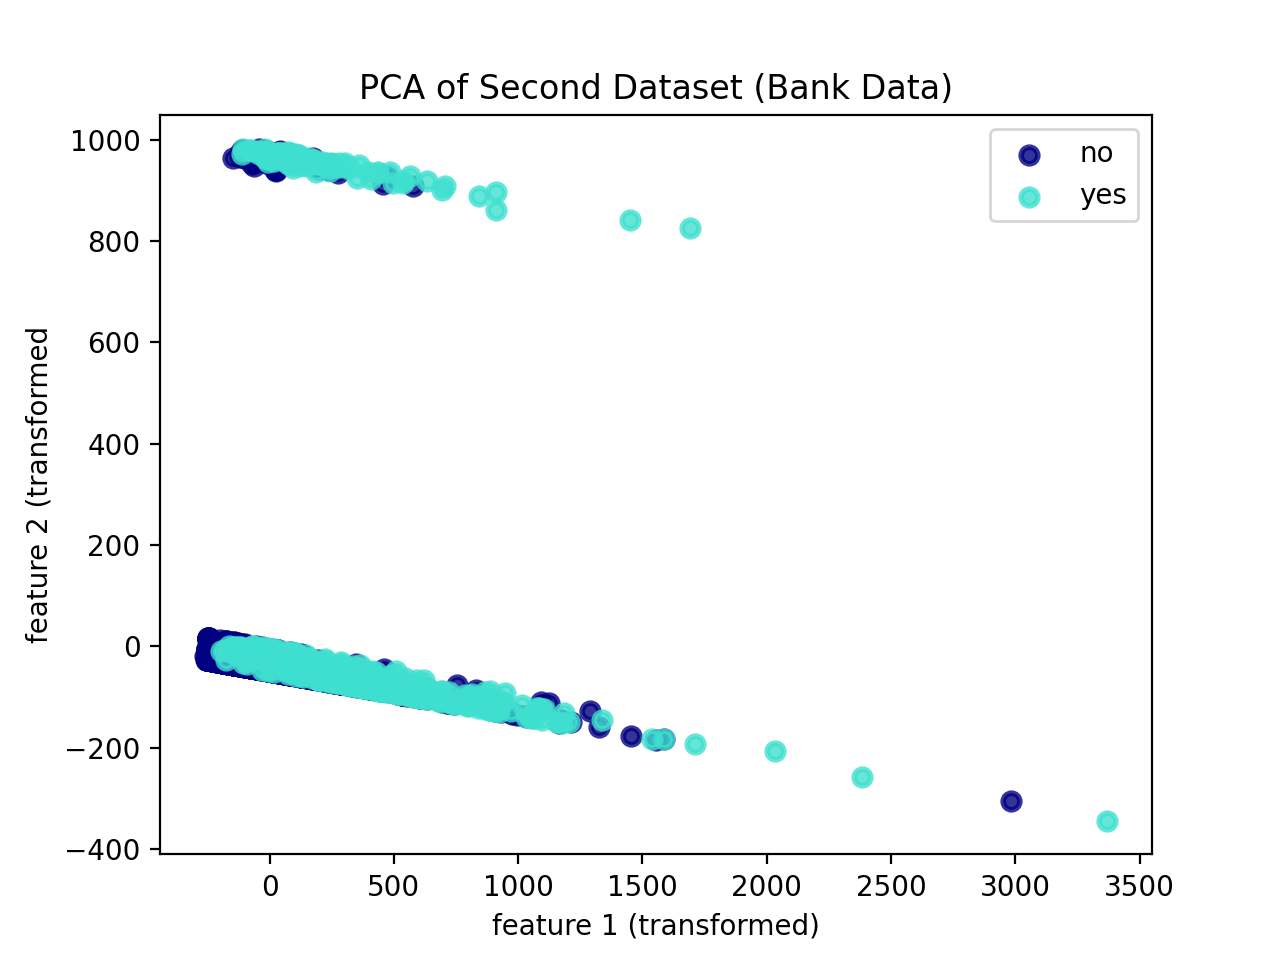
\includegraphics[width=.9\linewidth]{pcads2.png}
        \caption{DS1 Projection via PCA}\label{Fig:PCA DS2}
    \end{minipage}
\end{figure}

\subsection{Independent Components Analysis}\label{subsec:independent-components-analysis}
Similar to the previous I also attempted to search for the best number of components for each dataset.
According to Carsten Klein\cite{klein_2019}
"An interesting thing about two independent, non-Gaussian signals is that their sum is more Gaussian than any of the source signals.
Therefore we need to optimize W in a way that the resulting signals of Wx are as non-Gaussian as possible."
In other words, using a measurement like Kurtosis we can compare the "Gaussianity" of different ICA runs.
Since the normal distribution (Gaussian) has a kurtosis of 3, we are searching for ICA components with kurtosis of < 3.
In order to reduce the covariance of the feature vectors as much as possible (to in effect ensure they were independent
components, I elected to whiten the feature space before processing.)
Below is a table depicting the n-components selected for each dataset and the resulting Kurtosis.
\begin{itemize}
    \item For ICA, how kurtotic are the distributions?
    \item Do the projection axes for ICA seem to capture anything "meaningful"?
\end{itemize}
\begin{figure}
    \begin{minipage}{0.5\textwidth}
        \centering
        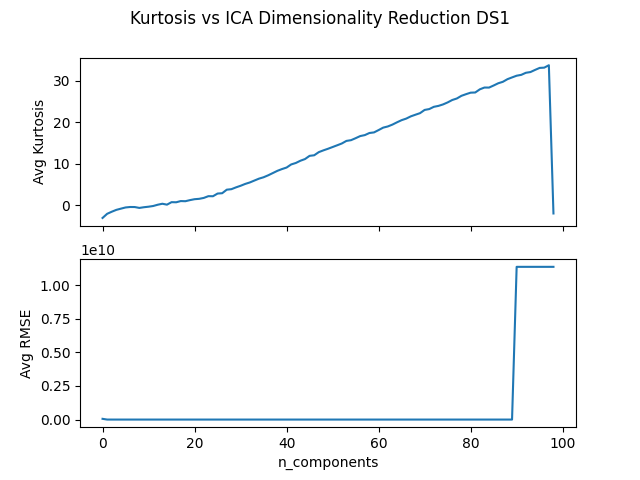
\includegraphics[width=.9\linewidth]{icads1.png}
        \caption{ICA Kurtosis vs RCError DS1}\label{Fig:ICA DS1}
    \end{minipage}\hfill
    \begin{minipage}{0.5\textwidth}
        \centering
        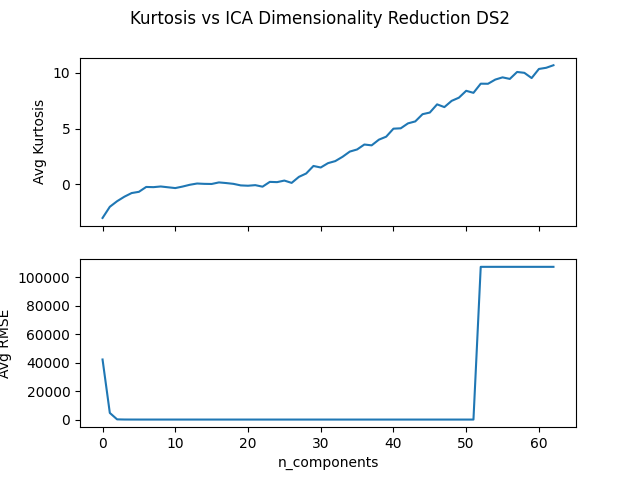
\includegraphics[width=.9\linewidth]{icads2.png}
        \caption{ICA Kurtosis vs RCError DS2}\label{Fig:ICA DS2}
    \end{minipage}
\end{figure}

\subsection{Randomized Projection}\label{subsec:randomized-projection}
\begin{itemize}

    \item Assuming you only generate k projections (i.e., you do dimensionality reduction), how well is the data reconstructed by the randomized projections? PCA?
    \item How much variation did you get when you re-ran your RP several times (I know I don't have to mention that you might want to run RP many times to see what happens, but I hope you forgive me)?
\end{itemize}
\begin{center}
    \begin{tabular}{|c| c |c|}
        \hline
        & Variance               & Standard Deviation \\
        \hline
        \hline
        Dataset 1 & 5.4456097845336664e+16 & 233358303.57057506 \\
        \hline
        Dataset 2 & 34540925361.18495      & 185851.89092711688 \\
        \hline
    \end{tabular}
\end{center}
\begin{figure}
    \begin{minipage}{0.5\textwidth}
        \centering
        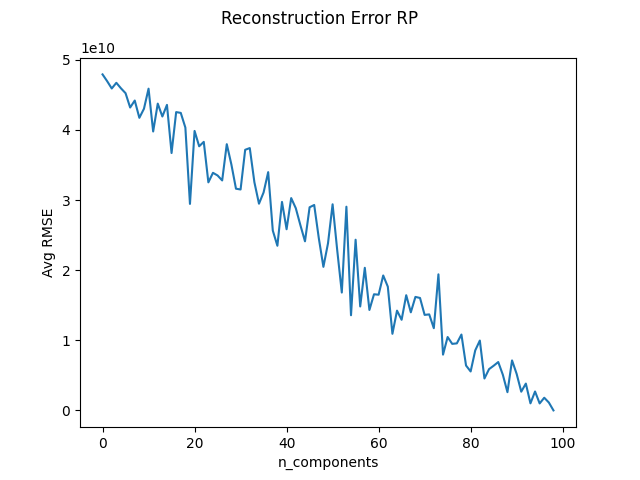
\includegraphics[width=.9\linewidth]{rpds1.png}
        \caption{RCError RP DS1}\label{Fig:RP DS1}
    \end{minipage}\hfill
    \begin{minipage}{0.5\textwidth}
        \centering
        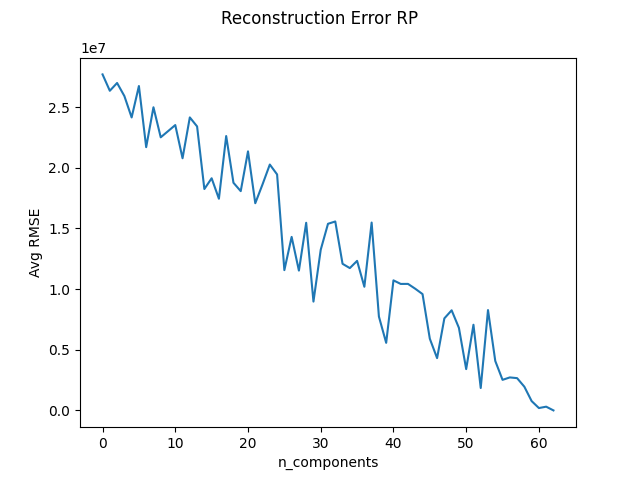
\includegraphics[width=.9\linewidth]{rpds2.png}
        \caption{RCError RP DS1}\label{Fig:RP DS2}
    \end{minipage}
\end{figure}

\subsection{Linear Discriminant Analysis}\label{subsec:linear-discriminant-analysis}
\begin{center}
    \begin{tabular}{|c| c |}
        \hline
        & Accuracy \\
        \hline
        \hline
        Dataset 1 & 82.86\%  \\
        \hline
        Dataset 2 & 91.17\%  \\
        \hline
    \end{tabular}
\end{center}